%\documentclass[12pt,a4paper,twoside]{article}
\documentclass[a4paper,twoside]{llncs}
\usepackage[utf8]{inputenc}
\usepackage{amsmath,amsfonts,amssymb}
\usepackage{graphicx}
\usepackage{algorithmic,algorithm}

\pagestyle{headings}%page numbers

\title{Generalised Rijndael}
\author{Sergi Blanch-Torn\'e\inst{1}, Ramiro Moreno Chiral\inst{2}, Francesc Seb\'e Feixa\inst{2}}
 \institute{
 Escola Polit\`ecnica Superior, Universitat de Lleida. Spain.\\
 \email{\tt sblanch@alumnes.udl.es}
 \and 
 Departament de Matem\`atica. Universitat de Lleida. Spain.\\
 \email{\tt \{ramiro,fsebe\}@matematica.udl.es}
 }

%%% abreviaturas matem\'aticas
% Enteros
\newcommand{\Z}{\ensuremath{\mathbb{Z}}} 

% Anillo de los enteros mod n
\newcommand{\Zn}[1]{\ensuremath{\mathbb{Z}/#1\mathbb{Z}}} 

% Cuerpo finito de orden p (primo)
\newcommand{\Fq}[1]{\ensuremath{\mathbb{F}_#1}} 

% Cuerpo finito de caractar\'{\i}stica p, grado n
\newcommand{\Fpn}[2]{\ensuremath{\mathbb{F}_{#1^#2}}} 

% Anillo polinomial con coeficientes en un cuerpo polinomial binario
\newcommand{\Fpnm}[2]{\ensuremath{\frac{\Fpn{2}{#1}[#2]}{m(#2)}}}

\renewcommand{\algorithmicrequire}{\textbf{INPUT:}}%
\renewcommand{\algorithmicensure}{\textbf{OUTPUT:}}%
\renewcommand{\algorithmiccomment}[1]{/* #1 */}%	

\floatname{algorithm}{Algorithm}%
\floatname{definition}{Definition}%

\begin{document}
\maketitle
\begin{center}
 \today
\end{center}

\begin{abstract}\footnote{Partially founded by the Spanish project MTM20\_\_-\_\_\_\_\_-\_\_\_-\_\_}
 This is the abstract
% this article comes from a real request, for small block cipher, but the tuneable paramenters in rijndael creates the idea to, further than an small version, it can be generalized
\\\\    
{\bf Keywords:} Cryptography, Symmetrics, Rijndael
\end{abstract}

%%%%%%%%%%%%%%%%
\section{Introduction}
% There are many other options of symmetric ciphers with different block sizes. AES is very static, but rijndael allows to play with paramenters. AESwrap (rfc3394) can be mention as another possibility.
% problem aproach (rijndael scalability)
% alternative cryptosystems
\cite{Daemen:1998:BCR:646692.759487}
\cite{Daemen98aesproposal:}
\cite{rfc3394}
\cite{AES-FIPS}


%%%%%%%%%%%%%%%%
\section{Approach to the Rijndael Schema}
% what is a PRP? and why is Rijndael a secure PRP?
\begin{definition}\label{def:PRP}
 A PseudoRandom Permutation (PRP) is defined as a application from the message space $\mathcal{M}$ and the key space $\mathcal{K}$ to the cipher space $\mathcal{C}$:
 \begin{center}
  \begin{tabular}{llll}
   PRP: & $\mathcal{M} \times \mathcal{K}$ & $\rightarrow$ & $\mathcal{C}$ \\
  \end{tabular}
 \end{center}
 such that:
 \begin{enumerate}
  \item $\exists$ ``efficient'' algorithm $c=E(k,m)$
  \item $\exists$ ``efficient'' inverse such that $m=D(k,c)$
  \item The functions $E$ and $D$ are one-to-one
 \end{enumerate}
\end{definition}

Consider an scenario where an adversary has access to a random oracle where the output of this oracle can be or the output of the PRP or a truly random output, the advantage of the adversary to distinguish between if the output is get from one or the other can be described as:
\begin{equation}\label{eq:prpAdv}
 {Adv}_{F}^{prp} = Pr[{Exp}_{F}^{r}(A)=1]-Pr[{Exp}_{F}^{prp}(A)=1]
\end{equation}
where ${Exp}_{F}^{r}$ represents an experiment of the truly random output and ${Exp}_{F}^{prp}$ the same but with the PRP.

\begin{definition}\label{def:securePRP}
 A PRP is secure if for all ``efficient'' adversary if the advantage to distinguish if the output is from the PRP or the truly random is ``negligible''
\end{definition}

The most efficient attacks on Rijndael      that means this algorithm is still secure.

% rijndael good characteristics
% shannon: confusion & diffusion => substitution & permitation
% structure of the input (fix block size)
% format preserving encryption alternative?

%%%%%%%%%%%%%%%%
\subsection{Design}
% what is the state matrix
% describe the transformations from the Shammir ``confussion and diffusion'' point of view.

%%%%%%%%%%%%%%%%
\section{Generalising the schema}

%TODO: Draw the procedure as diagram
\begin{figure}[h]
 \centering
 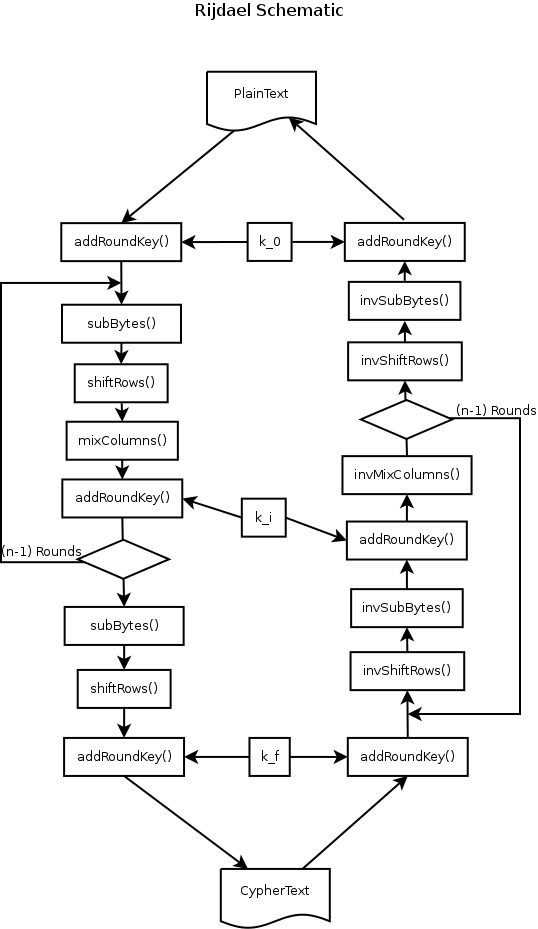
\includegraphics[scale=0.5,keepaspectratio=true]{./images/rijndaelDiagram.png}
 % rijndaelDiagram.png: 521x887 pixel, 72dpi, 18.38x31.29 cm, bb=0 0 521 887
 \caption{rijndael diagram}
 \label{fig:RijndaelDiagram}
\end{figure}


%%%%%%%%%%%%%%%%
\subsection{key expansion}
% abstraction of what it is, independent from the #rows, #columns, wordsize
% subBytes() is used, then the sboxes but is explained later on.
% when key n#columns is different than message #columns

\begin{algorithm}
 \caption{KeyExpansion}
 \label{alg:keyExpansion}
 \begin{algorithmic}[1]
  \REQUIRE byte k[nRows*nColumns], nRounds, nRowns, nColumns, wSize
  \ENSURE word w[nRouns*(nRows+1)]
  \STATE i := 0
  \WHILE{i<nColumns}
    \STATE w[i] := word(k[nRows*(i+c) for c in range(nColumns)])
  \ENDWHILE
  \STATE i := nColumns
  \WHILE{i<nRouns*(nRows+1)}
    \STATE temp := w[i-1]
    \IF{i mod nColumns == 0}
      \STATE temp := SubWord(RotWord(temp)) $\oplus$ Rcon[i/nColumns]
    \ELSE
      \STATE temp := SubWord(temp)
    \ENDIF
    \STATE w[i] := w[i-nColumns] $\oplus$ temp
    \STATE i++
  \ENDWHILE
 \end{algorithmic}
\end{algorithm}

% draw the algorithm as a diagram
\begin{figure}[b]
 \centering
 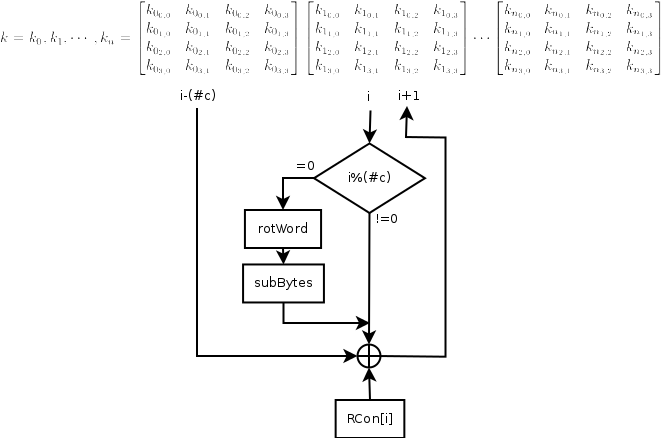
\includegraphics[scale=0.5,keepaspectratio=true]{./images/rijndael_keyExpansionDiagram.png}
 % rijndael_keyExpansionDiagram.png: 661x438 pixel, 72dpi, 23.32x15.45 cm, bb=0 0 661 438
 \caption{Block diagram of the construction of the rijndael key expansion}
\label{fig:keyExpansionDiagram}
\end{figure}


%%%%%%%%%%%%%%%%
\subsection{Rounds}
% why n rounds and not more, not less?

%%%%%%%%%%%%%%%%
\subsection{subBytes}
% abstraction of what it is, independent from the #rows, #columns, wordsize
% operations in the polynomial field F_{2^w} w: wordsize
%TODO: draw schematic of this step

%%%%%%%%%%%%%%%%
\subsubsection{How to build different SBoxes}
% how the sbox was build and how to build a new one with different parameters
\begin{figure}[h]{\tiny
\begin{center}
\begin{tabular}[]{|l||l|l|l|l|l|l|l|l|l|l|l|l|l|l|l|l|}\hline
    & 0x0  & 0x1  & 0x2  & 0x3  & 0x4  & 0x5  & 0x6  & 0x7  & 0x8  & 0x9  & 0xA  & 0xB  & 0xC  & 0xD  & 0xE  & 0xF \\\hline\hline
0x0 & 0x63 & 0x7C & 0x77 & 0x7B & 0xF2 & 0x6B & 0x6F & 0xC5 & 0x30 & 0x01 & 0x67 & 0x2B & 0xFE & 0xD7 & 0xAB & 0x76\\\hline
0x1 & 0xCA & 0x82 & 0xC9 & 0x7D & 0xFA & 0x59 & 0x47 & 0xF0 & 0xAD & 0xD4 & 0xA2 & 0xAF & 0x9C & 0xA4 & 0x72 & 0xC0 \\\hline
0x2 & 0xB7 & 0xFD & 0x93 & 0x26 & 0x36 & 0x3F & 0xF7 & 0xCC & 0x34 & 0xA5 & 0xE5 & 0xF1 & 0x71 & 0xD8 & 0x31 & 0x15 \\\hline
0x3 & 0x04 & 0xC7 & 0x23 & 0xC3 & 0x18 & 0x96 & 0x05 & 0x9A & 0x07 & 0x12 & 0x80 & 0xE2 & 0xEB & 0x27 & 0xB2 & 0x75 \\\hline
0x4 & 0x09 & 0x83 & 0x2C & 0x1A & 0x1B & 0x6E & 0x5A & 0xA0 & 0x52 & 0x3B & 0xD6 & 0xB3 & 0x29 & 0xE3 & 0x2F & 0x84 \\\hline
0x5 & 0x53 & 0xD1 & 0x00 & 0xED & 0x20 & 0xFC & 0xB1 & 0x5B & 0x6A & 0xCB & 0xBE & 0x39 & 0x4A & 0x4C & 0x58 & 0xCF \\\hline
0x6 & 0xD0 & 0xEF & 0xAA & 0xFB & 0x43 & 0x4D & 0x33 & 0x85 & 0x45 & 0xF9 & 0x02 & 0x7F & 0x50 & 0x3C & 0x9F & 0xA8 \\\hline
0x7 & 0x51 & 0xA3 & 0x40 & 0x8F & 0x92 & 0x9D & 0x38 & 0xF5 & 0xBC & 0xB6 & 0xDA & 0x21 & 0x10 & 0xFF & 0xF3 & 0xD2 \\\hline
0x8 & 0xCD & 0x0C & 0x13 & 0xEC & 0x5F & 0x97 & 0x44 & 0x17 & 0xC4 & 0xA7 & 0x7E & 0x3D & 0x64 & 0x5D & 0x19 & 0x73 \\\hline
0x9 & 0x60 & 0x81 & 0x4F & 0xDC & 0x22 & 0x2A & 0x90 & 0x88 & 0x46 & 0xEE & 0xB8 & 0x14 & 0xDE & 0x5E & 0x0B & 0xDB \\\hline
0xA & 0xE0 & 0x32 & 0x3A & 0x0A & 0x49 & 0x06 & 0x24 & 0x5C & 0xC2 & 0xD3 & 0xAC & 0x62 & 0x91 & 0x95 & 0xE4 & 0x79 \\\hline
0xB & 0xE7 & 0xC8 & 0x37 & 0x6D & 0x8D & 0xD5 & 0x4E & 0xA9 & 0x6C & 0x56 & 0xF4 & 0xEA & 0x65 & 0x7A & 0xAE & 0x08 \\\hline
0xC & 0xBA & 0x78 & 0x25 & 0x2E & 0x1C & 0xA6 & 0xB4 & 0xC6 & 0xE8 & 0xDD & 0x74 & 0x1F & 0x4B & 0xBD & 0x8B & 0x8A \\\hline
0xD & 0x70 & 0x3E & 0xB5 & 0x66 & 0x48 & 0x03 & 0xF6 & 0x0E & 0x61 & 0x35 & 0x57 & 0xB9 & 0x86 & 0xC1 & 0x1D & 0x9E \\\hline
0xE & 0xE1 & 0xF8 & 0x98 & 0x11 & 0x69 & 0xD9 & 0x8E & 0x94 & 0x9B & 0x1E & 0x87 & 0xE9 & 0xCE & 0x55 & 0x28 & 0xDF \\\hline
0xF & 0x8C & 0xA1 & 0x89 & 0x0D & 0xBF & 0xE6 & 0x42 & 0x68 & 0x41 & 0x99 & 0x2D & 0x0F & 0xB0 & 0x54 & 0xBB & 0x16 \\\hline
\end{tabular}
\end{center}}
\caption{Sbox for 8 bits word size}
\label{tab:sbox8}
\end{figure}


%%%%%%%%%%%%%%%%
\subsection{shiftColumns}
% abstraction of what it is, independent from the #rows,GeneralizedRijndael/sboxes.py #columns, wordsize
%TODO: draw schematic of this step

%%%%%%%%%%%%%%%%
\subsection{mixColumns}
% abstraction of what it is, independent from the #rows, #columns, wordsize
% polynomial ring, where the coeficients are elements from a binary polynomial field
%   \Fpnm{x}{z}, ord(m)=#rows
%   (this is, in mho, one of the most important points of rijndael)
%TODO: draw schematic of this step
\subsection{Operate in a polinomial ring, with coeficients in a polinomial field}
$$\Fpnm{n}{y}\label{eq:polinomialRing}$$ where $m(y)$ is a composed polinomial of degree $r$ columns. This gives a polinomial ring. The coeficients of this polinomial ring are elements of a polinomial field $$\Fpn{2}{n}=\Fpnm{2}{x}\label{eq:polinomialField}$$ where $m(x)$ is irreductible and gives a polinomial field.
Standard rijndael (AES) uses a circulan invertible matrix for this to simplify and speed up the operations in the ring.

%%%%%%%%%%%%%%%%
\subsection{addRoundKey}
% the operation where the key is used (from the 4 rijndael operations)
% simply a xor operation (addition in F_2)
%TODO: draw schematic of this step

%%%%%%%%%%%%%%%%
\section{Parameter combinations}
% how, with different parameters, can have the same block sizes, and what's different between them

%%%%%%%%%%%%%%%%
\section{New useful sizes for Rijndael}
% because of the newer processors with 64 bits, it can be easy to have bigger sizes with less costs
\cite{Daemen:1999:EBC:1267115.1267119}

%%%%%%%%%%%%%%%%
%TODO: what else should be in the paper?
% \section{Attacking the schema}
% 
% \subsection{Side channel attacks}
% %?difference between precalculated sbox and rcon or compute on the fly
% % constant time operation intervals and equivalent memory use
% % key expansion calculated during the encrypt/decrypt process
% \section{Conclusions}

%%%%%%%%%%%%%%%%
\bibliographystyle{ieeetr}
\bibliography{../bibtex/sblanch.bib,../bibtex/standards.bib,../bibtex/symmetrics.bib,../bibtex/rijndael.bib,../bibtex/books.bib,../bibtex/crypto.bib,../bibtex/rfc.bib}

\end{document}